\section{Remaining systematics}\label{sec:systests}

\begin{figure*}
\centering
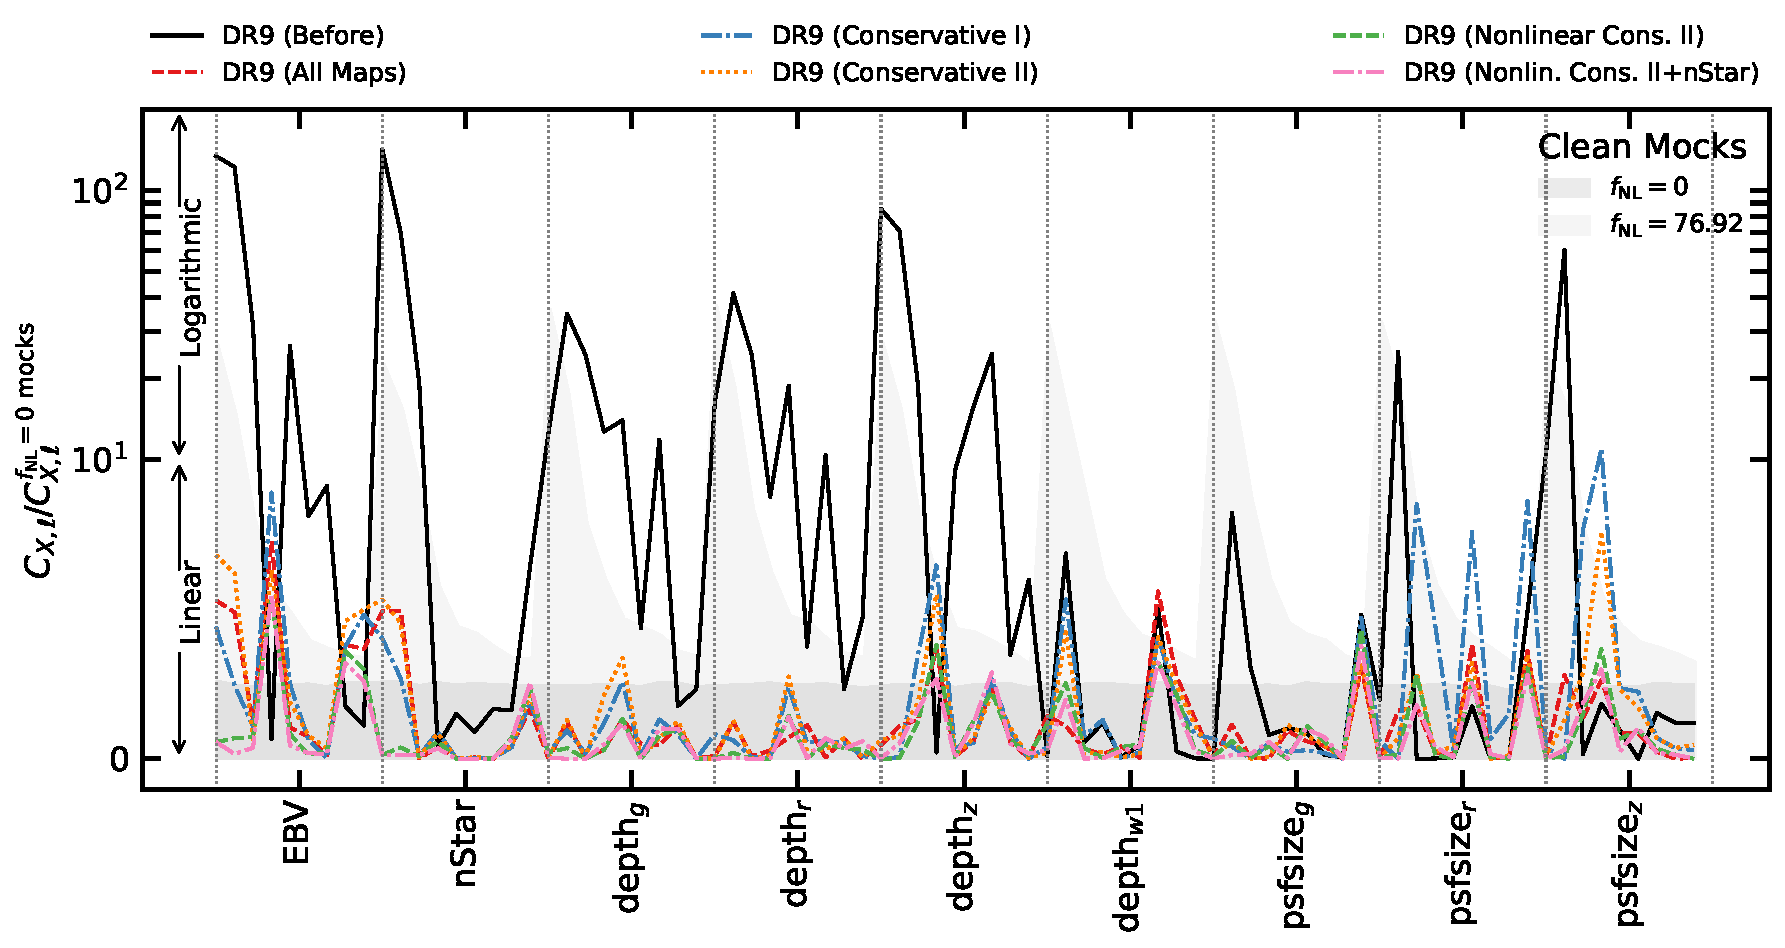
\includegraphics[width=0.95\textwidth]{clx_mocks.pdf}
\caption{The square of the cross power spectra between the DESI LRG targets and imaging systematic maps normalized by the auto power spectrum of the imaging systematic maps; see equation \ref{eq:cx}. The systematic maps considered are Galactic extinction (EBV), stellar density (nStar), depth in \textit{grzw1} (depth$_{grzw1}$), and seeing in \textit{grz} (psfsize$_{grz}$). The black curves display the cross spectra before imaging systematic correction. The red, blue and orange curves represent the results after applying the imaging weights from the linear models trained with \textit{eight maps}, \textit{two maps}, and \textit{three maps}. The green and pink curves display the results after applying the imaging weights from the non-linear models trained with \textit{three maps} and \textit{four maps}. The dark and light shades represent the $97.5$ percentile from cross correlating the imaging systematic maps and the $\fnl=0$ and $76.9$ lognormal density fields, respectively.}\label{fig:clxmock}
\end{figure*}

\begin{figure*}
\centering
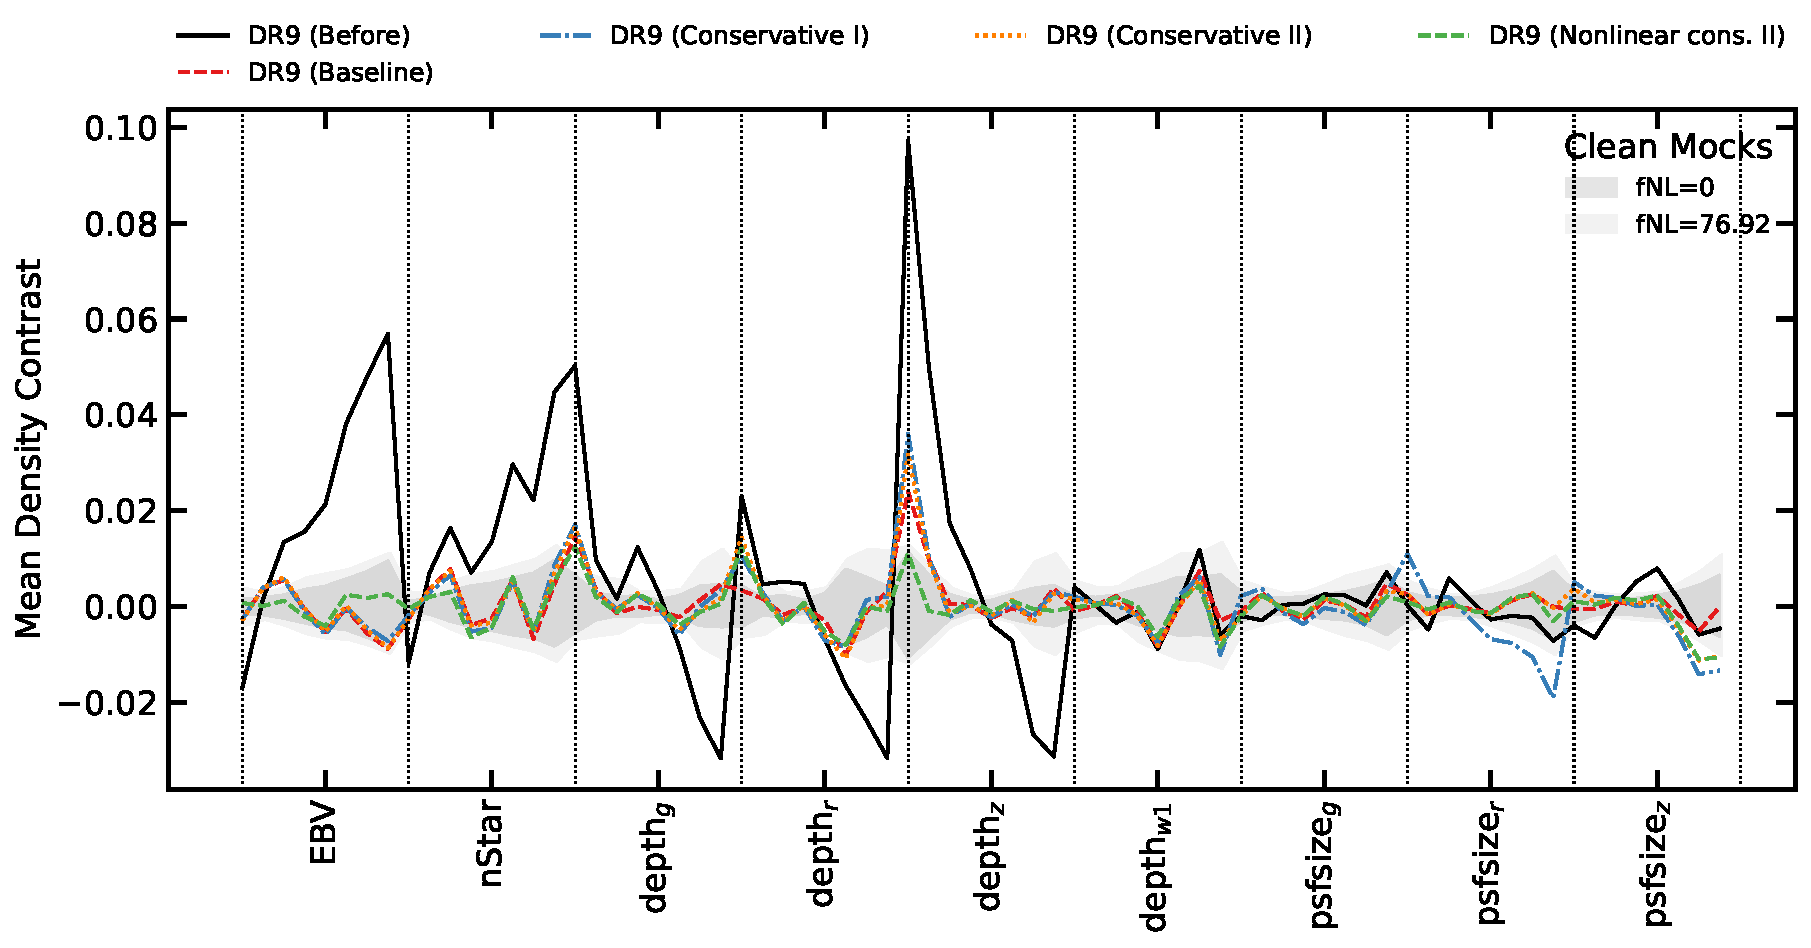
\includegraphics[width=0.95\textwidth]{nbar_mocks.pdf}
\caption{The mean density contrast of the DESI LRG targets as a function of the imaging systematic maps: Galactic extinction (EBV), stellar density (nStar), depth in \textit{grzw1} (depth$_{grzw1}$), and seeing in \textit{grz} (psfsize$_{grz}$). The black curves display the results before imaging systematic correction. The red, blue and orange curves represent the relationships after applying the imaging weights from the linear models trained with \textit{two maps}, \textit{three maps}, and \textit{eight maps}, respectively. The green and pink curves display the results after applying the imaging weights from the non-linear models trained with \textit{three maps} and \textit{four maps}. The dark and light shades represent the $68\%$ dispersion of 1000 lognormal mocks with $\fnl=0$ and $76.9$, respectively.}\label{fig:nbarmock}
\end{figure*}

\subsection{Cross power spectrum}

We characterize the cross correlations between the galaxy density and imaging systematic maps by
\begin{equation}
\tilde{C}_{X, \ell} = [\tilde{C}_{x_{1}, \ell}, \tilde{C}_{x_{2}, \ell}, \tilde{C}_{x_{3}, \ell}, ..., \tilde{C}_{x_{9}, \ell}],
\end{equation}
where $\tilde{C}_{x_{i}, \ell}$ represents the the square of the cross power spectrum between the galaxy density and $i^{\rm th}$ imaging map, $x_{i}$, divided by the auto power spectrum of $x_{i}$:
\begin{equation}\label{eq:cx}
\tilde{C}_{x_{i}, \ell} = \frac{(\tilde{C}_{gx_{i}, \ell})^{2}}{\tilde{C}_{x_{i}x_{i},\ell}}.
\end{equation}
With this normalization, $\tilde{C}_{x_{i}, \ell}$ estimates the contribution of systematics at every multipole up to the linear order to the galaxy power spectrum. Then, the $\chi^{2}$ value for the cross power spectra is calculated via,
\begin{equation}\label{eq:cx_chi2}
\chi^{2} = \tilde{C}^{T}_{X, \ell} \mathbb{C}_{X}^{-1} \tilde{C}_{X, \ell},
\end{equation}
where the covariance matrix $\mathbb{C}_{X} = < \tilde{C}_{X, \ell} \tilde{C}_{X, \ell'} >$ is constructed from the lognormal mocks \mr{with $\fnl=0$}. These $\chi^{2}$ values are measured for every clean mock realization with the \textit{leave-one-out} technique and compared to the values observed in the DESI LRG targets with various imaging systematic corrections. Specifically, we use 999 realizations to estimate a covariance matrix and then apply the covariance matrix from the 999 realizations to measure the $\chi^{2}$ for the one remaining realization. This process is repeated for all 1000 realizations to construct a histogram for $\chi^{2}$. We only include the bandpower bins from $\ell=2$ to $20$ with $\Delta\ell=2$, which results in a total of 81 bins, and test for the robustness with higher $\ell$ modes in Appendix \ref{sec:scalesys}. 

Figure \ref{fig:clxmock} shows $\tilde{C}_{X,\ell}$ from the DESI LRG targets before and after applying various corrections for imaging systematics. The dark and light shades show the 97.5$^{\rm th}$ percentile from the $\fnl=0$ and $76.9$ mocks, respectively. Without imaging weights, the DESI LRG targets have the highest cross-correlations against extinction, stellar density, and depth in z (solid black curve). There are less significant correlations against depth in the g and r bands, and psfsize in the z band, which could be driven because of the inner correlations between the imaging systematic maps. First, we consider cleaning the DESI LRG targets with the linear model using two maps (extinction and depth in z) as identified from the Pearson correlation. Linear two maps is the most conservative systematic treatment method in terms of both the model flexibility and the number of input maps. With linear two maps (red dashed curve), most of the cross correlation signals are reduced below statistical uncertainties, especially against extinction, stellar density, and depth. However, the cross correlations against psfsize in r and z increases slightly on $6<\ell<20$ and $6<\ell<14$, respectively. 

Regression against extinction and depth in the z-band helps mitigate large-scale cross correlations ($\ell < 6$), but there are some residual power on smaller scales ($\ell > 6$) which cannot be mitigated with our set of two maps. The linear three maps (blue dot-dashed curve) approach alleviates the cross correlation against psfsize in r, and it yields similar results to those obtained from \textit{linear eight maps}, which indicates no further information can be extracted from eight maps using the linear approach. Therefore, we identify extinction, depth in z, and psfsize in r (\textit{three maps}) as the primary sources of systematic effects in the DESI LRG targets. Then, we adapt \textit{neural network three maps} to model non-linear systematic effects. Compared with the linear three maps method, we find that non-linear three maps (green dashed curve) can reduce the cross correlations against both the r and z-band psfsize maps, which shows the benefit of using a non-linear approach. To further examine the robustness of our cleaning methods, we also show the cross correlations after cleaning the DESI LRG targets with linear eight maps (orange dotted curve) and non-linear four maps (pink dot-dashed curve). 

\subsection{Mean density contrast}

We calculate the histogram of the mean density contrast relative to the $j^{\rm th}$ imaging property, $x_{j}$:
\begin{equation}
\delta_{x_{j}} = ({\overline{\rho}})^{-1} \frac{\sum_{i} \rho_{i} W_{i}}{\sum_{i} W_{i}} \mr{- 1},
\end{equation}
where $\overline{\rho}$ is the global mean galaxy density, $W_{i}$ is the survey window in pixel $i$, and the summations over $i$ are evaluated from the pixels in every bin of $x_{j}$. We compute the histograms against all nine imaging properties (see Figure \ref{fig:ng}). We use a set of eight equal-width bins for every imaging map, which results in a total of 72 bins. Then, we construct the total mean density contract as,
\begin{equation}
\delta_{X} = [\delta_{x_{1}}, \delta_{x_{2}}, \delta_{x_{3}}, ..., \delta_{x_{9}}],
\end{equation}
and the total residual error as,
\begin{equation}
\chi^{2} = \delta_{X}^{T} \mathbb{C_{\delta}}^{-1} \delta_{X},
\end{equation}
where the covariance matrix $\mathbb{C}_{\delta} = < \delta_{X} \delta_{X}>$ is constructed from the lognormal mocks \mr{with $\fnl=0$ that have had no mitigation applied to them}. Figure \ref{fig:nbarmock} shows the mean density contrast against the imaging properties for the DESI LRG targets. The dark and light shades represent the $1\sigma$ level fluctuations observed in 1000 lognormal density fields respectively with $\fnl=0$ and $76.9$. The DESI LRG targets before treatment (solid curve) exhibits a strong trend around $10\%$ against the z-band depth which is consistent with the cross power spectrum. Additionally, there are significant spurious trends against extinction and stellar density at about $5-6\%$. The linear approach is able to mitigate most of the systematic fluctuations with only extinction and depth in the z-band as input; however, a new trend appears against the r-band psfsize map with the \textit{linear two maps} approach (red dashed curve), which is indicative of the psfsize-related systematics in the DESI LRG targets. This finding is in agreement with the cross power spectrum. We re-train the linear model with three maps, but we still observe around $2\%$ residual spurious fluctuations in the low end of depth$_{z}$ and around $1\%$ in the high end of psfsize$_{z}$, which implies the presence of non-linear systematic effects. We find that the imaging weights from the non-linear model trained with the three identified maps (or four maps including the stellar density) are capable of reducing the fluctuations below $2\%$. Even with the non-linear three maps, we have about $1\%$ remaining systematic fluctuations against the z-band psfsize. We use the $\chi^{2}$ statistics to assess how significant these fluctuations are in comparison to the clean mocks. 

\begin{figure}
\raggedright
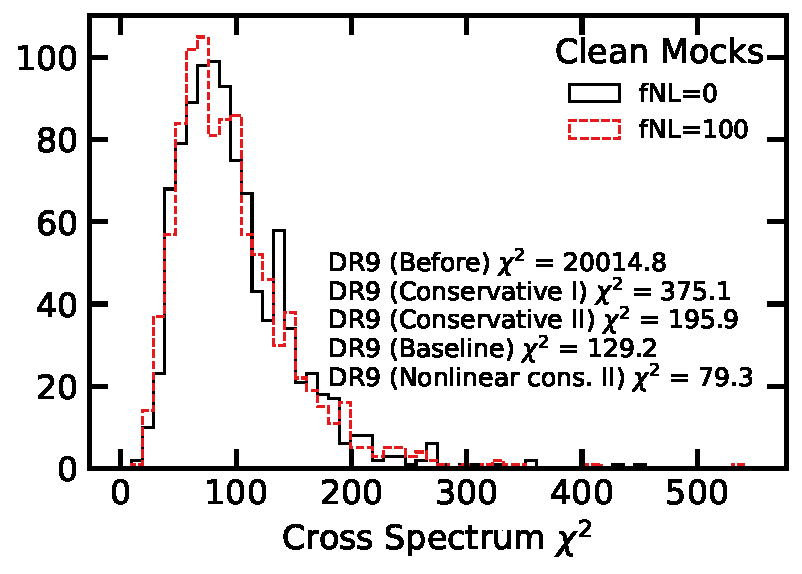
\includegraphics[width=0.45\textwidth]{chi2test.pdf}
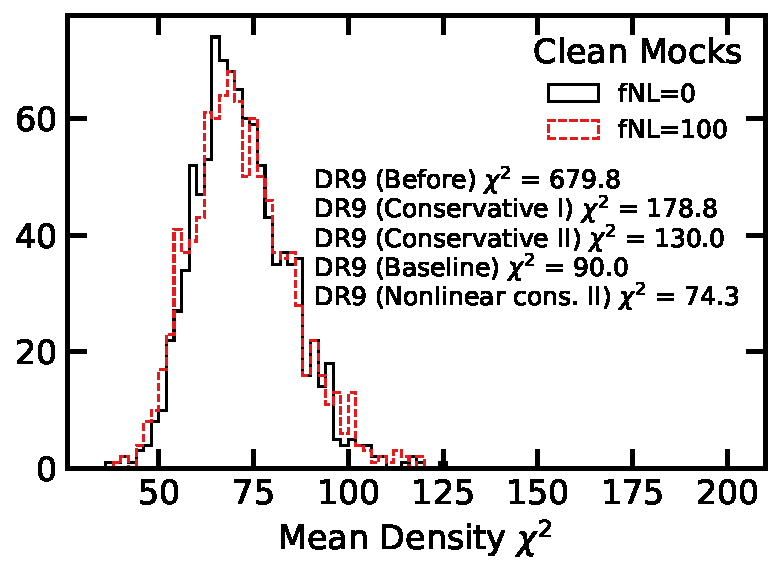
\includegraphics[width=0.44\textwidth]{chi2test2.pdf}
\caption{The remaining systematic error $\chi^{2}$ from the galaxy-imaging cross power spectrum (top) and the mean galaxy density contrast (bottom). The values observed in the DESI LRG targets before and after linear and non-linear treatments are represented via vertical lines, and the histograms are constructed from 1000 realizations of clean lognormal mocks with $\fnl=0$ and $76.9$.}\label{fig:chi2test}
\end{figure}

Figure \ref{fig:chi2test} presents $\chi^{2}$ histograms for the normalized cross spectrum (top) and mean density contrast (bottom) statistics obtained from lognormal mocks with different $\fnl$ values. \mout{The $\chi^{2}$ tests are insensitive to $\fnl$, providing consistent distributions regardless of its value that was used for mock generation, and thus these tests help separate systematics from cosmology.} No mitigation is applied to the mocks, ensuring unbiased $\chi^{2}$ values. DESI LRG target $\chi^{2}$ values are compared via the vertical lines and summarized in Table \ref{tab:chi2test}. After cleaning, the cross power spectrum's $\chi^{2}$ is reduced. However, linear three maps approach fails to clean the data properly at $95\%$ confidence ($\chi^{2}=195.9$ and $p$-value $< 0.04$). Alternative non-linear three maps approach reduces $\chi^{2}$ significantly with $p$-value $=0.59$, supporting the need for non-linear cleaning. For this test, we only use multipoles for up to $\ell=20$, and we find no remaining systematic errors by investigating at higher multipoles (see Appendix \ref{sec:scalesys}). We observe similar performance in the mean density test. The \textit{linear two maps} weights reduce the $\chi^{2}$ from $679.8$ to $178.8$, but significant systematics remain ($p$-value $<0.001$). Applying the linear three maps approach lowers the error to $\chi^{2}=130$, yet systematics remain significant ($p$-value $<0.001$). Cleaning with linear eight maps results in $\chi^{2}=90$ and $p$-value $=0.08$, but using too many imaging maps increases the risk of removing the true clustering signal. Alternatively, using imaging weights from the \textit{non-linear three maps} approach yields $\chi^{2}=74.3$ and $p$-value $=0.39$. Adding the stellar density map (\textit{non-linear four maps}) slightly improves the results: $\chi^{2}=73.2$ and $p$-value $=0.42$. The small impact on $\chi^{2}$ suggests that the stellar density trend can be explained by extinction due to the correlation between these properties, such that in regions with high stellar density, there is likely to be a higher concentration of dust, which can cause greater extinction of light. \mr{The non-linear method with nine maps is our most aggressive treatment which results in the lowest residual errors, $\chi^{2}=39.7$ ($p$-value = $>0.99$) and $49.1$ ($p$-value = $0.88$), respectively, for the mean density and cross-power spectrum statistics.}
\begin{table}
  \caption{Mean density and cross power spectrum $\chi^{2}$ and $p$-values that are inferred from the comparison to the $\fnl=0$ clean mocks \mr{that have had no mitigation applied to them}.}\label{tab:chi2test}
  \begin{tabular}{lcccc}
    \hline
    \hline
    \multirow{2}{*}{\textbf{Method}} &
      \multicolumn{2}{c}{\textbf{Mean Density}} &
      \multicolumn{2}{c}{\textbf{Cross Spectrum}} \\
    & $\chi^{2}$ & $p$-value & $\chi^{2}$ & $p$-value \\
    \hline
   No Weight & 679.8 & < 0.001 & 20014.8 & < 0.001 \\
   Linear Two Maps & 178.8 & < 0.001 & 375.1 & < 0.001 \\
   Linear Three Maps & 130 & < 0.001  & 195.9 & 0.04 \\
   Linear Eight Maps & 90 & 0.08  & 129.2 & 0.24 \\
   Nonlinear Three Maps & 74.3 & 0.39  & 79.3 & 0.59 \\
   Nonlinear Four Maps & 73.2 & 0.42  & 70.9 & 0.69\\  
   \mr{Nonlinear Nine Maps} & \mr{39.7} & \mr{> 0.99 } & \mr{49.1} & \mr{0.88}\\
    \hline
  \end{tabular}
\end{table}

The tests conducted here demonstrate the effectiveness of various cleaning approaches for the DESI LRG targets without revealing the measured power spectrum or $\fnl$ constraints. Results summarized in Table \ref{tab:chi2test} show that cleaning with non-linear three maps consistently produces $\chi^{2}$ values similar to clean mocks with reasonable $p$-values ($=0.39$ for mean density and $=0.59$ for cross power spectrum). On the other hand, the linear three maps approach fails to sufficiently mitigate systematics, as evidenced by low $p$-values ($< 0.001$ for mean density and $=0.04$ for cross power spectrum). Considering $p=0.05$ as a threshold for clean maps, the non-linear three maps approach is optimal, as adding more imaging systematic maps may exacerbate over-correction issues. \mr{When we compare the mean density $\chi^{2}$ from the DESI LRG targets to the $\fnl=0$ mocks that have had the same imaging mitigation applied, we find that both nonlinear three and four maps have not entered the regime of over-correction. Whereas, nonlinear nine maps has reached the level of over-correction. This is illustrated in Figure \ref{fig:chi2scatter}.}

\begin{figure}
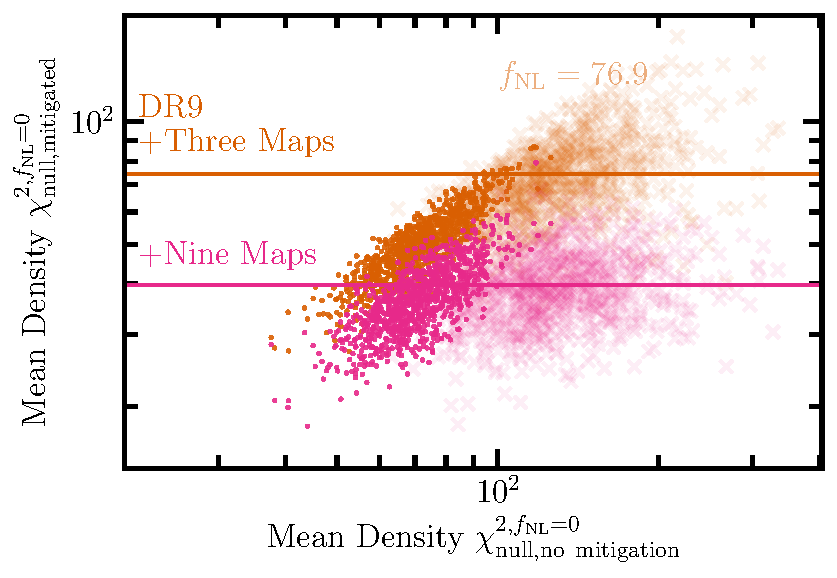
\includegraphics[width=0.5\textwidth]{chi2_scatter.pdf}
\caption{\mr{The remaining systematic error $\chi^{2}$ from the mean galaxy density contrast for mocks with $\fnl=0$ before (shown on horizontal scale) and after mitigation (shown on vertical scale) using the nonlinear three (orange), four (purple), and nine maps (pink) cleaning methods. The faded orange squares represent the values observed in the $\fnl=76.9$ mocks after nonlinear three maps. The values observed in the DESI LRG targets after the same treatments are shown with solid lines.}}\label{fig:chi2scatter}
\end{figure}


\mr{Figure \ref{fig:chi2scatter} illustrates the remaining systematic error $\chi^{2}$ from the mean density contrast for mocks with $\fnl=0$ before (shown on horizontal scale) and after mitigation (shown on vertical scale) using the nonlinear three, four, and nine maps cleaning methods. The values for the $\fnl=76.9$ mocks are shown for nonlinear three maps only. The values observed in the DESI LRG targets after the same treatments are shown with solid lines. Note that the covariance matrices for the mean density and cross power spectrum are based on the $\fnl=0$ mocks. As a result, we find that the $\chi^{2}$ values for the $\fnl=76.9$ mocks are significantly larger than that of the $\fnl=0$ realizations. Therefore, these $\chi^{2}$ tests will have a preference for correction until excess power is removed, or equivalently, $\fnl=0$ is recovered even if the underlying $\fnl$ of the Universe is non-zero. We also find that the differences are resilient against log transformation, and we cannot make the $\chi^{2}$ tests insensitive to the $\fnl$ value that is used in the mocks.} 

\mr{As shown in Figure \ref{fig:contmcmc}, we are able to recover the true $\fnl$ using the coefficients derived in Table \ref{ssec:calibration}. The associated drawback is that statistical precision will be diminished due to the large-scale clustering information being removed by mitigating with more maps than necessary. Our work motivates better diagnostics for the characterization of systematic error, such that it robustly differentiates large-scale excess power due to imaging systematics from that of non-zero local PNG.}




\section{Extra robustness tests}

\mr{\subsection{Survey window convolution}\label{ssec:windowconv}
Here we calculate the mode-mode coupling matrix from the DESI mask. This matrix depends only on the survey geometry and can be described in terms of the window power spectrum \citep{hivon2002master},}
\begin{equation}
M_{\ell \ell^{\prime}} = \frac{2\ell^{\prime}+1}{4\pi} \sum_{\ell^{\prime\prime}} (2\ell^{\prime\prime}+1) \tilde{C}^{\rm window}_{\ell^{\prime\prime}} \begin{pmatrix}
\ell & \ell^{\prime} & \ell^{\prime\prime}\\
0 & 0 & 0
\end{pmatrix},
\end{equation}
\mr{where the last term in the right hand side represents the Wigner 3-j symbol (or Clebsch-Gordan coefficient), and is calculated using \textsc{SymPy} \citep{sympy2017}. We benchmark our code against the publicly available software, \textsc{NaMaster}\footnote{\href{https://github.com/LSSTDESC/NaMaster}{https://github.com/LSSTDESC/NaMaster}} \citep{2019MNRAS.484.4127A}. Figure \ref{fig:window_conv} illustrates the different approaches to account for the mode-mode coupling caused by the DESI survey window for two arbitrary values of $\fnl$. The red shade represents the 68\% dispersion of the $\fnl=76.9$ mocks.}


\begin{figure}
    \centering
    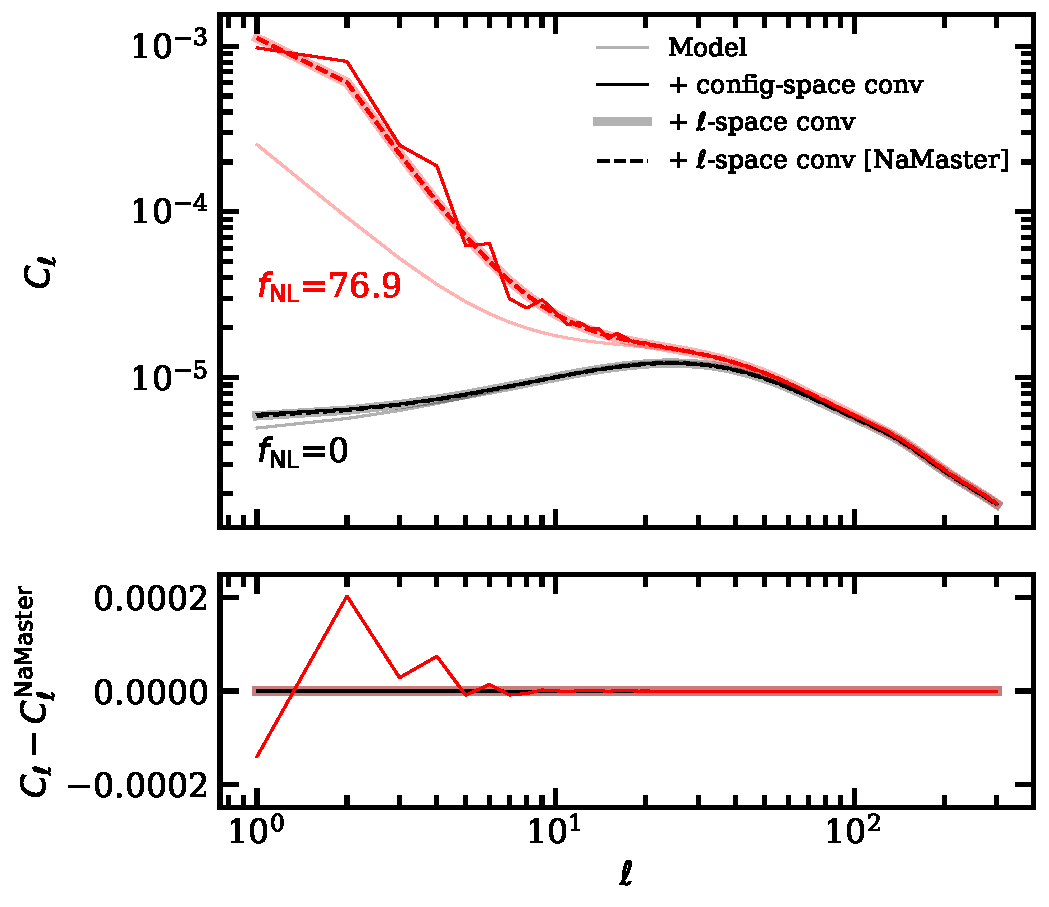
\includegraphics[width=0.5\textwidth]{figures/cl_conv.pdf}
    \caption{\mr{The model power spectrum before and after the survey geometry convolution for $\fnl=0$ and $76.9$ using the DESI survey mask. The bottom panel shows the residual error with respect to the \textsc{NaMaster} code. The shade represents the dispersion of the $\fnl=76.9$ mocks.}}
    \label{fig:window_conv}
\end{figure}

\subsection{Scale dependent systematics}\label{sec:scalesys}
Our fiducial cross power spectrum diagnostic (equation \ref{eq:cx_chi2}) uses harmonic modes up to $\ell=20$, which determines the smallest scale used for characterizing residual systematic errors. To investigate the statistical significance of the cross power spectrum's $\chi^{2}$, we examine its dependence on the largest harmonic mode $\ell_{\rm max}$. We extend $\ell_{\rm max}$ from $20$ to $100$, where the latter scale corresponds to density fluctuations on scales smaller than $2$ degrees. Figure \ref{fig:chi2cellextend} shows the median of the cross power spectrum's $\chi^{2}$ from the clean $\fnl=0$ mocks as the highest mode $\ell_{\rm max}$ increases from $20$ to $100$ (represented by the solid line). The red circles and blue crosses show the $\chi^{2}$ values for the DESI LRG targets cleaned respectively with the linear and neural network approaches, both with three maps. Overall, we find that for all scales up to $\ell=100$, the nonlinear three maps approach yields consistent values with the clean mocks, whereas the linear three maps approach exhibits significant remaining systematics at more than 95\% confidence.

\begin{figure}
\centering
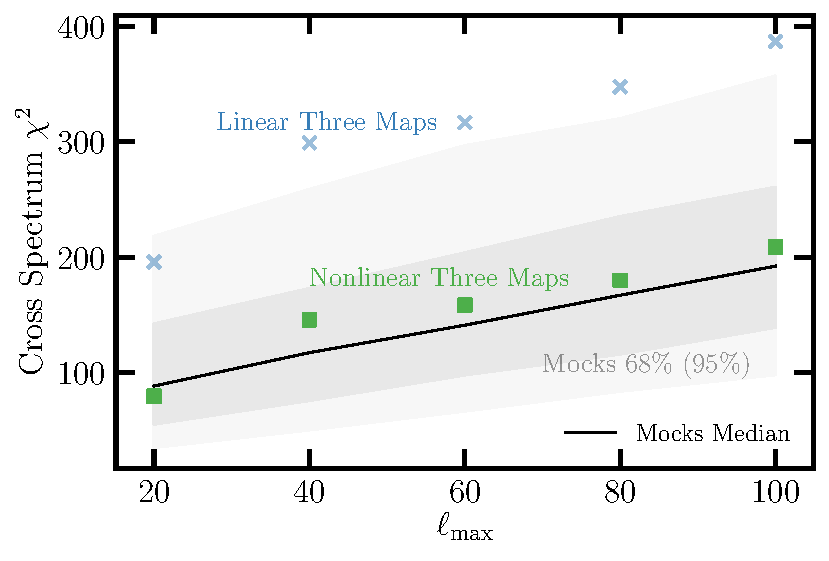
\includegraphics[width=0.5\textwidth]{chi2lmax.pdf}
\caption{The cross power spectrum's $\chi^{2}$ between the DESI LRG target density and imaging systematic maps as a function of the highest mode $\ell_{\rm max}$ when the sample is cleaned with the linear (triangles) and non-linear (squares) three maps. The lowest mode is fixed at $\ell_{\rm min}=2$. The solid curve and dark (light) shade represent the median value and $68\%$ ($95\%$) confidence regions, estimated from the $\fnl=0$ mocks.}\label{fig:chi2cellextend}
\end{figure}


\subsection{Redshift uncertainties}\label{ssec:nzuncer}

\begin{figure}
\raggedleft
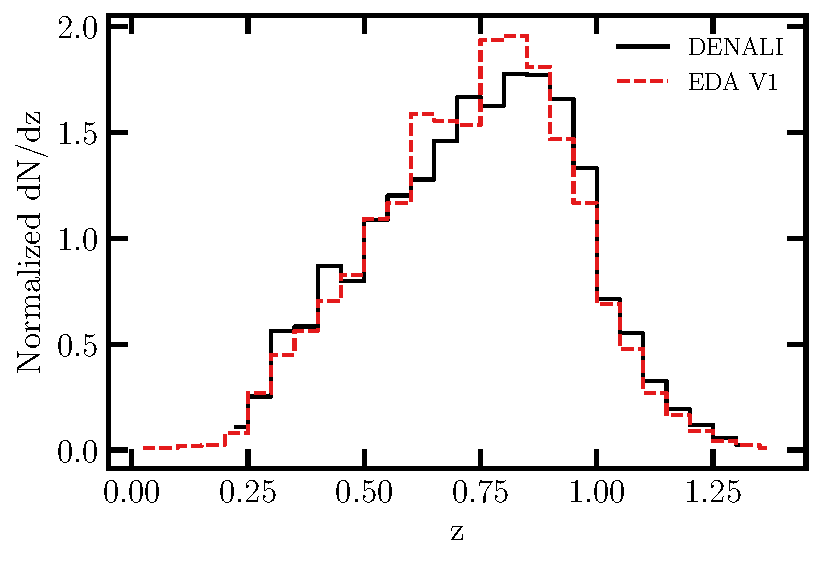
\includegraphics[width=0.46\textwidth]{figures/nz_lrg_eda.pdf}
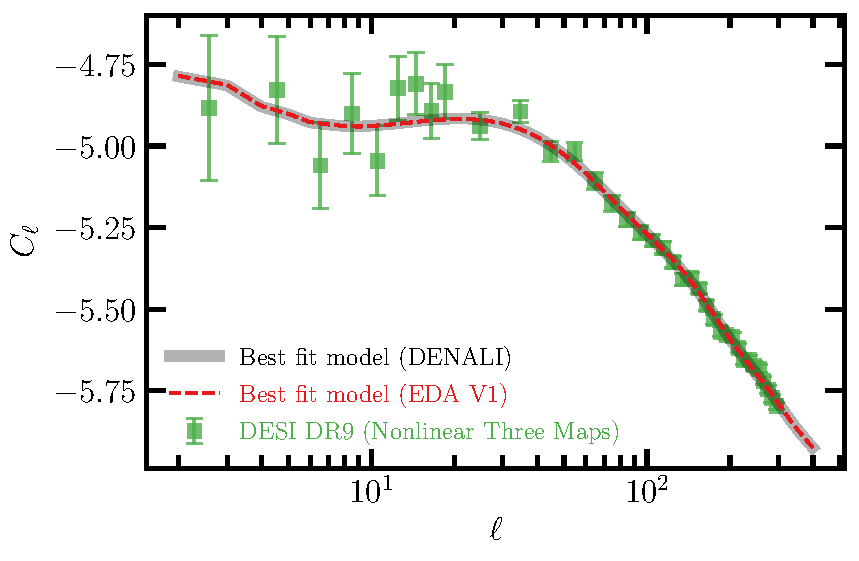
\includegraphics[width=0.48\textwidth]{figures/cl_nz.pdf}\caption{Top: The redshift distribution of the DESI LRG targets from the EDA V1 and Denali. Bottom: The measured power spectrum of the DESI LRG targets and the best fit theory models using different redshift distributions.}\label{fig:cl_nz}
\end{figure}

We use the Early Data Assembly Version 1 (EDA V1) to construct the redshift distribution for the DESI LRG targets. We find that the change in the maximum likelihood estimate of $\fnl$ is negligible, \mr{$|\Delta \fnl | < 1$, compared to the statistical precision of our measurements}. Figure \ref{fig:cl_nz} shows the measured power spectrum of the DESI targets and the corresponding best fit theory curves. The variations in $dN/dz$ do not significicantly alter the conclusion of our paper.

\subsection{Spurious bump in NGC}\label{ssec:ndecalsbump}

\begin{figure}
    \centering
    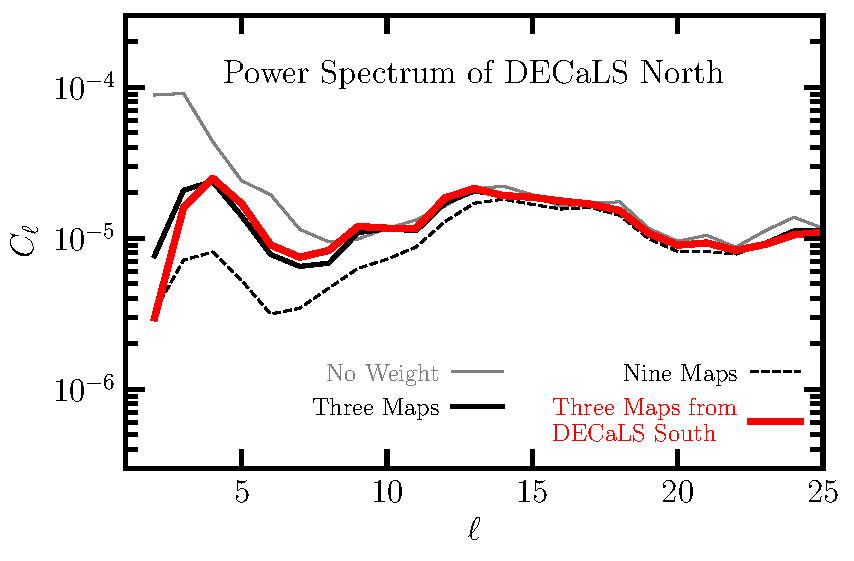
\includegraphics[width=0.48\textwidth]{figures/cl_SonN.pdf}
    \caption{The unbinned measured power spectrum of the DESI LRG targets in the DECaLS North region before and after various mitigations using the neural network approach.}
    \label{fig:clSonN}
\end{figure}

As shown in Figure \ref{fig:mcmc_dr9elmin} (top panel), we realize that the spurious feature at $\ell \sim 10-20$ is removed in the DECaLS South region after mitigation, but it remains in the BASS+MzLS and DECaLS North. We use the neural networks trained on the DECaLS South with three and nine maps to mitigate the galaxy density in the DECaLS North region, and then measure the power spectrum. Figure \ref{fig:clSonN} shows the power spectrum before treatment (No Weight) and after the nonlinear three maps and nine maps methods for comparison. We find that whatever causing the bump is different between the DECaLS North and South. The best-fit estimates for $\fnl$ from the DR9 DECaLS North using the neural network correction with three maps (NN trained on DECaLS North), three maps (NN trained on DECaLS South), and nine maps (NN trained on DECaLS South) are $41$, \mr{$36$}, and \mr{$75$}, respectively. \mr{The solution without correction (No weight) results in a best fitting estimate of $\fnl=94$.}


\section{Lognormal mocks}

We fit the mean power spectrum of the lognormal mocks to validate the modeling pipeline, and in particular the survey geometry and integral constraint treatments. We investigate the impact of covariance matrix on the inference of $\fnl$. Finally, we show the impact of imaging systematic mitigation and the over-subtraction effect when the cleaning methods are applied to the mocks. 

\subsection{Clean mocks}
The $68\%$ and $95\%$ probability contours on the PNG parameter $\fnl$ and bias coefficient $b$ are shown in Figure \ref{fig:mcmc_mocks0} and \ref{fig:mcmc_mocks100}, respectively, for the $\fnl=0$ and 76.9 mocks. The best-fitting, marginalized mean estimates, as well as the $1\sigma$ and $2\sigma$ confidence intervals of $\fnl$ are summarized in Table \ref{tab:mocksmcmc}. 

Measuring the power spectrum from the entire DESI footprint reduces the cosmic variance and thus improves the constraining power. Figure \ref{fig:mcmc_mocks0} compares the constraints from fitting the log of the mean power spectrum of the mocks when it is measured from the DESI footprint to those obtained from the sub imaging surveys. We find that the underlying true $\fnl$ value is recovered within $95\%$ confidence, and that the contours for the DESI region are smaller by a factor of two. 

\begin{figure}
    \centering
    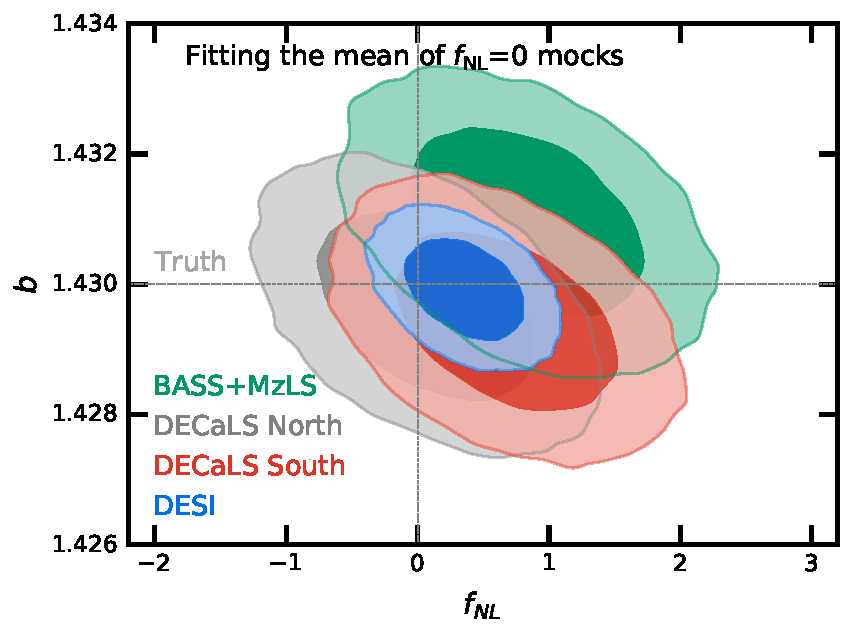
\includegraphics[width=0.48\textwidth]{figures/mcmc_zero.pdf} 
    \caption{68\% and 95\% confidence contours from the mean power spectrum of the $\fnl=0$ mocks for the DESI footprint and sub-imaging surveys. The truth values are represented by vertical and horizontal lines.}\label{fig:mcmc_mocks0}
\end{figure}

\begin{figure}
    \centering
    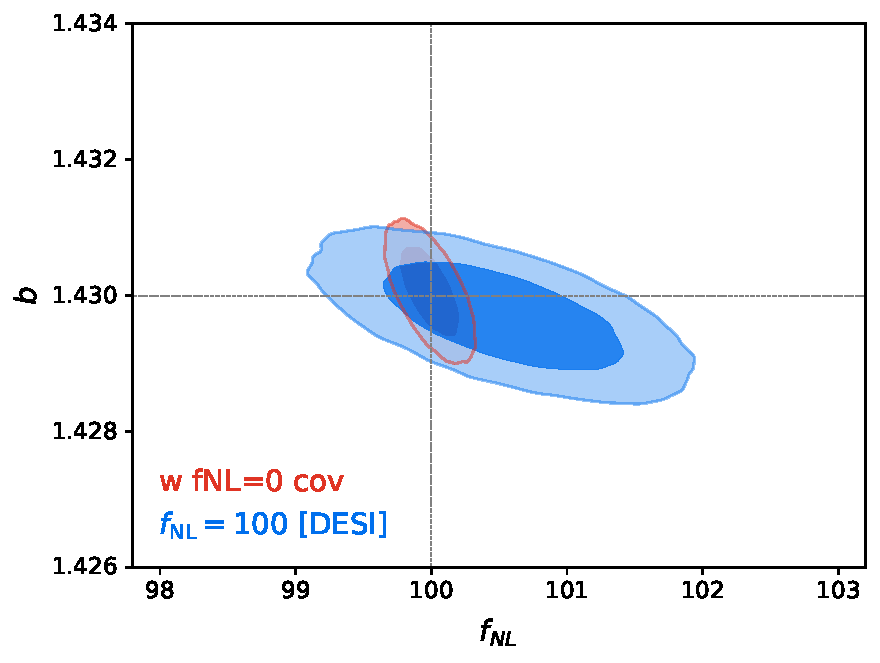
\includegraphics[width=0.48\textwidth]{figures/mcmc_po100.pdf} 
    \caption{68\% and 95\% confidence contours of fitting the mean power spectrum or its log transformation from the $\fnl=76.9$ mocks for the DESI footprint. Using the $\log C_{\ell}$ fitting yield constraints that are insensitive to the covariance used. The truth values are represented by vertical and horizontal lines.}\label{fig:mcmc_mocks100}
\end{figure}

\begin{figure}
    \centering
    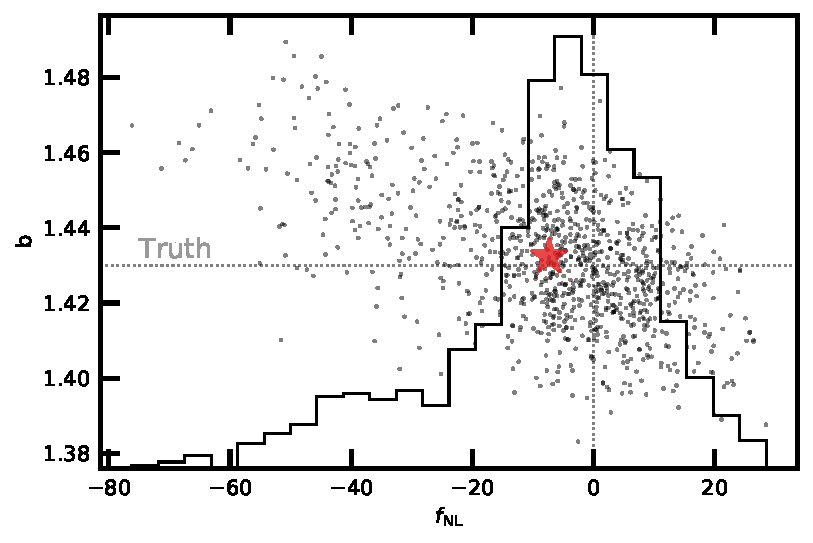
\includegraphics[width=0.45\textwidth]{figures/bestfit_zero.pdf} 
    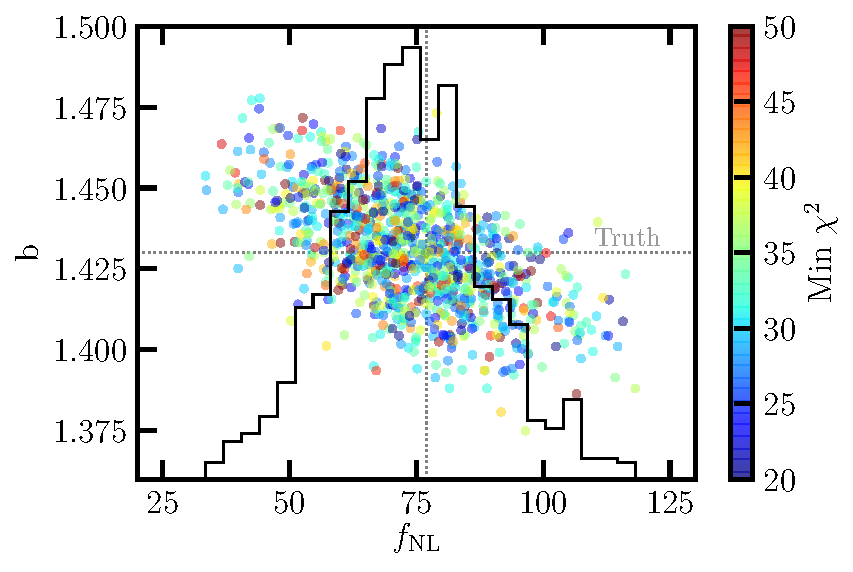
\includegraphics[width=0.45\textwidth]{figures/bestfit_po100.pdf}         
    \caption{The best-fitting estimates of $b$ and $\fnl$ from fitting 1000 lognormal mocks with $\fnl=0$ (top) and $76.9$ (bottom) in the DESI footprint. No mitigation is applied to the mocks. The truth values are represented by vertical and horizontal lines.}\label{fig:bestfit_mocks}
\end{figure}

The power spectrum of the mocks at low $\ell$ is very sensitive to the cosmic variance and the true value of $\fnl$. Consequently, a large value of $\fnl$ can induce very large power on low $\ell$, and thus significantly change the covariance matrix. We find that applying the log transformation on the power spectrum makes the result more robust against the choice of the covariance matrix. Figure \ref{fig:mcmc_mocks100} shows the confidence contours when we fit either the power spectrum or its log transform of the $\fnl=76.9$ mocks, and use different covariance matrices. We consider the $\fnl=0$ and $76.9$ mocks to construct the covariance from one set and use it to fit the mean power spectrum of the other set. When the covariance matrix is constructed from the same set of mocks used for the mean power spectrum, we find that the difference in $\fnl$ constraints between fitting the power spectrum and its log transformation is negligible at only 2\%. If we use the $\fnl=0$ mocks to estimate the covariance, and fit the log power spectrum of the $\fnl=76.9$ mocks, we find that the error on $\fnl$ increases only by $7\%$. However, when the mean power spectrum of the $\fnl=76.9$ mocks is fit using the covariance matrix estimated from the $\fnl=0$ mocks, the constraints tighten by a factor of $5$ due to a higher signal to noise ratio. Therefore, we argue that fitting the log power spectrum can help mitigate the need for having $\fnl$-dependent covariance matrices and make the constraints less sensitive to covariance construction.


\begin{table*}
    \caption{The best-fitting and marginalized mean estimates for $\fnl$ from fitting the mean power spectrum of the mocks. \mr{The covariance is scaled to represent the error on the mean power spectrum.} The number of degrees of freedom is 34 (37 data points - 3 parameters).}   
    \label{tab:mocksmcmc}  
   \centerline{%
    \begin{tabular}{llllllll}
    \hline
    \hline
   &  & & & & $\fnl$ &  \\
   \cmidrule(r{.7cm}){4-7}    
Mock / $\fnl$ &  Footprint   &  Observable & 	Best fit  & Mean & $ 68\%$ CL & $ 95\%$ CL & $\chi^{2}$ (dof $=34$)\\
    \hline
Clean $76.9$ & DESI & log$C_{\ell}$    & $ 77.67$& $ 77.67$& $ 77.17<\fnl< 78.16$& $ 76.71<\fnl< 78.64$ &   38.8\\
Clean $76.9$ & DESI & $C_{\ell}$       & $ 77.67$& $ 77.65$& $ 77.17<\fnl< 78.14$& $ 76.70<\fnl< 78.60$ &   39.0\\
Clean $76.9$ & DESI & log$C_{\ell}$ + $f_{\rm NL}=0$ cov & $ 77.70$& $ 77.71$& $ 77.25<\fnl< 78.17$& $ 76.81<\fnl< 78.63$ &   39.9\\
Clean $76.9$ & DESI & $C_{\ell}$ + $f_{\rm NL}=0$ cov & $ 77.03$& $ 77.02$& $ 76.93<\fnl< 77.12$& $ 76.83<\fnl< 77.22$ &  207.6\\
\hline
Clean $0$ & DESI         &  log$C_{\ell}$ & $  0.36$& $  0.36$& $  0.06<\fnl<  0.65$& $ -0.23<\fnl<  0.94$ &   35.7\\
Clean $0$ & BASS+MzLS    &  log$C_{\ell}$ & $  0.83$& $  0.82$& $  0.25<\fnl<  1.40$& $ -0.31<\fnl<  1.96$ &   39.4\\
Clean $0$ & DECaLS North &  log$C_{\ell}$& $  0.07$& $  0.06$& $ -0.47<\fnl<  0.60$& $ -1.00<\fnl<  1.12$ &   26.7\\
Clean $0$ & DECaLS South &  log$C_{\ell}$& $  0.67$& $  0.67$& $  0.13<\fnl<  1.22$& $ -0.40<\fnl<  1.75$ &   34.3\\
\hline
    \end{tabular}
    }
\end{table*}

Figure \ref{fig:bestfit_mocks} shows the best-fitting estimates for $b$ vs $\fnl$ for $\fnl=0$ and $=76.9$ mocks in the top and bottom panels, respectively. Truth values are represented via the dotted lines. The points are color-coded with the minimum $\chi^{2}$ from fit for each realization. The histograms of the best-fitting $\fnl$ estimates are plotted in the background. For the $\fnl=0$ mocks, the best-fitting estimates are more symmetric. To understand this behaviour, we consider the first derivative of the likelihood (Equation \ref{eq:likelihood}), which is proportional to the first derivative of the log power spectrum. By simplifying the integrals involved in $C_{\ell}$, we have $C_{\ell} = A_{0, \ell} + A_{1,\ell} \fnl + A_{2, \ell} \fnl^{2}$ where $A_{123,\ell}$ are $\ell$-dependent terms. Then, the derivative of the likelihood is proportional to
\begin{equation}
    \frac{d}{d\fnl}\log(C_{\ell}) = \frac{A_{1, \ell}+2A_{2, \ell}\fnl}{A_{0, \ell} + A_{1,\ell} \fnl + A_{2, \ell} \fnl^{2}}.
\end{equation}
For infinitesimal values of $\fnl$, the derivative becomes asymptotically independent from $\fnl$ while for large values of $\fnl$ it decreases as $2/\fnl$. This implies that for the $\fnl=0$ mocks, the likelihood is more likely to be skewed toward negative values.


\subsection{Contaminated mocks}\label{ssec:contmocks}
Our nonlinear neural network-based approach is applied to the $\fnl=0$ and $76.9$ mocks. We only consider the methods that include running the neural network with three, four, and nine imaging systematic maps. The measured mean power spectrum of the mocks are shown in Figure \ref{fig:clmocks} for $\fnl=0$ (left) and $76.9$ (right). The solid and dashed curves show the measurements respectively from the clean and contaminated mocks.

\begin{figure*}
    \centering
    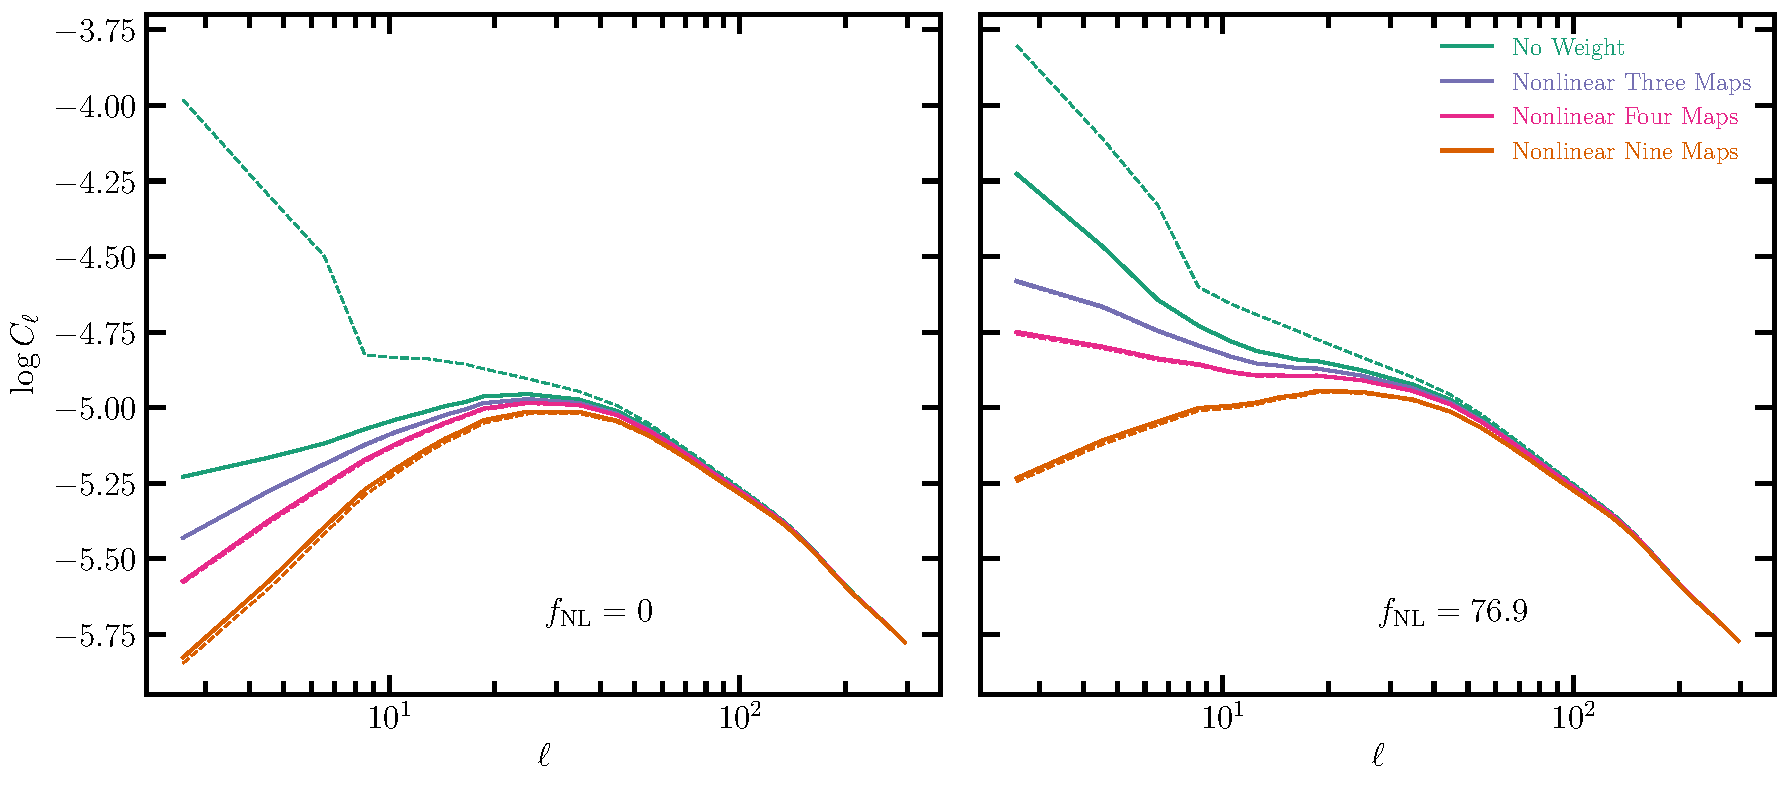
\includegraphics[width=0.9\textwidth]{figures/clmocks.pdf}
    \caption{The mean power spectrum of the $\fnl =0$ and $76.9$ mocks with (dashed) and without (solid) imaging systematics before ('No Weight') and after applying the non-linear cleaning method with three, four, and nine maps.}\label{fig:clmocks}
\end{figure*}


We find that the imaging treatment has removed some of the true clustering signal, and the amount of the over-subtraction is almost the same regardless of whether the mocks have systematics. The over-subtraction induces biases in the $\fnl$ constraints, as summarized in Table \ref{tab:contmocksmcmc}. The over-subtraction at low $\ell$ is so high that we get a poor fit after applying the mitigation with the nonlinear three maps approach, e.g., $\chi^{2}=86.8$ for the clean $\fnl=0$ mocks.


\begin{table*}
  %\begin{center}
    \caption{The best-fitting and marginalized estimates for $\fnl$ from fitting the mean power spectrum of the mocks before and after corrections using the non-linear approach with various combinations of the imaging systematic maps. \mr{The covariance is scaled to represent the error on the mean power spectrum.} The estimates are not accounted for over-correction, and therefore are subject to mitigation systematics.}   
    \label{tab:contmocksmcmc}  
   \centerline{%
    \begin{tabular}{lllllll}
    \hline
    \hline
   &  & 	   & & $\fnl$ + Mitigation Systematics & & \\
   \cmidrule(r{.7cm}){3-6}    
Mock / $\fnl$ & Method & Best fit  & Mean & $ 68\%$ CL & $ 95\%$ CL & $\chi^{2}$ (dof $=34$) \\
    \hline
Clean $0$ & No Weight                   & $  0.36$& $  0.36$& $  0.06<\fnl<  0.65$& $ -0.23<\fnl<  0.94$ &   35.7\\
Clean $0$ & Three Maps                  & $-11.64$& $-11.65$& $-12.00<\fnl<-11.30$& $-12.34<\fnl<-10.97$ &   86.8\\
Clean $0$ & Four Maps                   & $-20.14$& $-20.13$& $-20.44<\fnl<-19.82$& $-20.74<\fnl<-19.52$ &  472.8\\
Clean $0$ & Nine Maps                   & $-26.91$& $-26.92$& $-27.16<\fnl<-26.68$& $-27.39<\fnl<-26.46$ & 5481.0\\
Contaminated $0$ & Three Maps           & $-12.12$& $-12.13$& $-12.48<\fnl<-11.78$& $-12.83<\fnl<-11.44$ &   94.0\\
Contaminated $0$ & Four Maps            & $-20.97$& $-20.98$& $-21.28<\fnl<-20.67$& $-21.58<\fnl<-20.37$ &  556.3\\
Contaminated $0$ & Nine Maps            & $-28.13$& $-28.13$& $-28.36<\fnl<-27.90$& $-28.59<\fnl<-27.67$ & 6760.5\\
\hline
Clean $76.9$ & No Weight               & $ 77.67$& $ 77.67$& $ 77.17<\fnl< 78.16$& $ 76.71<\fnl< 78.64$ &   38.8\\
Clean $76.9$ & Three Maps              & $ 54.57$& $ 54.57$& $ 54.14<\fnl< 55.01$& $ 53.72<\fnl< 55.45$ &  603.5\\
Clean $76.9$ & Four Maps               & $ 38.38$& $ 38.38$& $ 37.99<\fnl< 38.78$& $ 37.60<\fnl< 39.16$ &  537.0\\
Clean $76.9$ & Nine Maps               & $  6.04$& $  6.04$& $  5.72<\fnl<  6.36$& $  5.41<\fnl<  6.67$ &  694.0\\
Contaminated $76.9$ & Three Maps       & $ 54.01$& $ 54.00$& $ 53.57<\fnl< 54.44$& $ 53.15<\fnl< 54.86$ &  588.0\\
Contaminated $76.9$ & Four Maps        & $ 37.48$& $ 37.49$& $ 37.09<\fnl< 37.88$& $ 36.70<\fnl< 38.27$ &  510.7\\
Contaminated $76.9$ & Nine Maps        & $  4.59$& $  4.58$& $  4.26<\fnl<  4.90$& $  3.95<\fnl<  5.22$ &  649.7\\
\hline
    \end{tabular}
    }
\end{table*}
Using the calibration parameters presented in \S \ref{ssec:calibration}, we account for the shift in the $\fnl$ constraints caused by the imaging systematic mitigation. We show the marginalized probability distributions on $\fnl$ before and after accounting for the over-correction in the right and left panels of Figure \ref{fig:contmcmc}.

\begin{figure*}
\centering
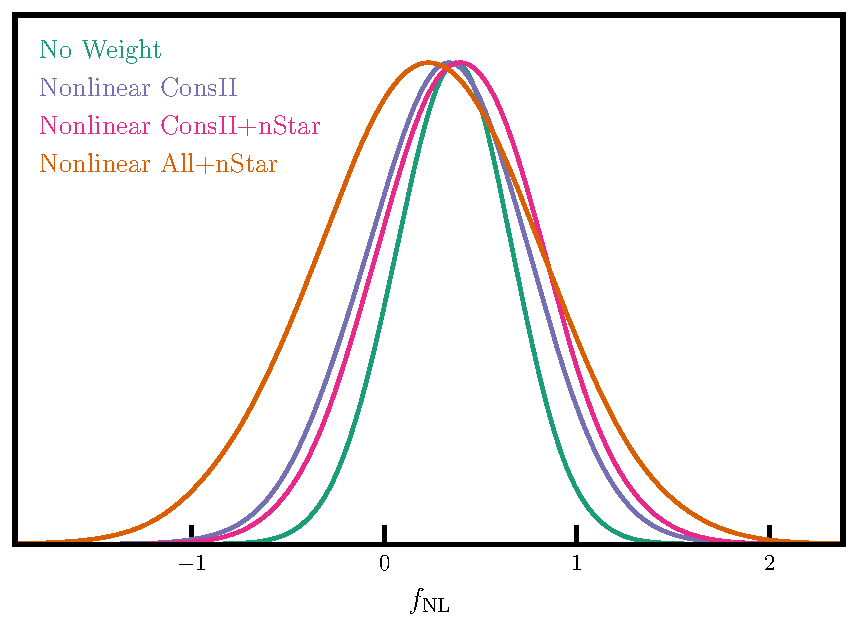
\includegraphics[width=0.45\textwidth]{figures/mcmc_cont.pdf}
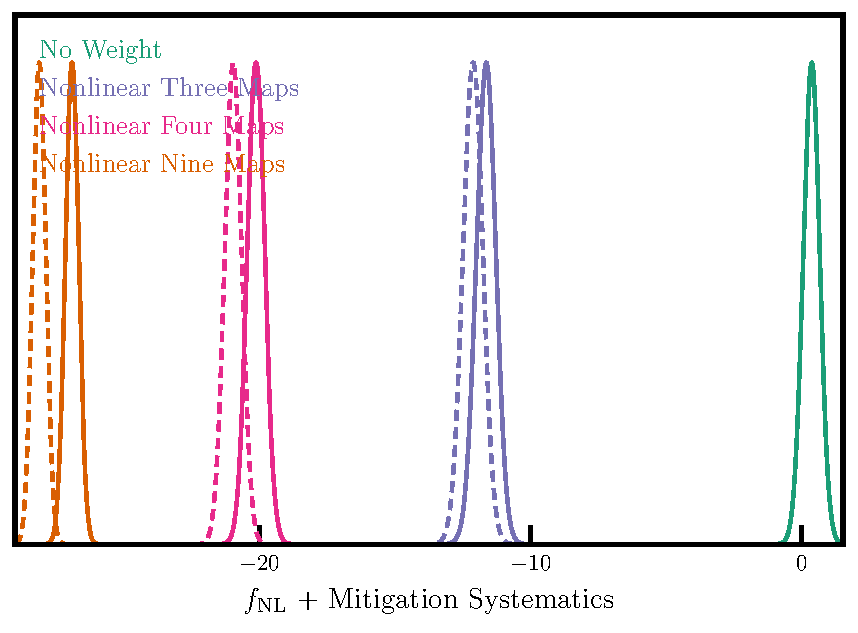
\includegraphics[width=0.45\textwidth]{figures/mcmc_contnoshift.pdf}
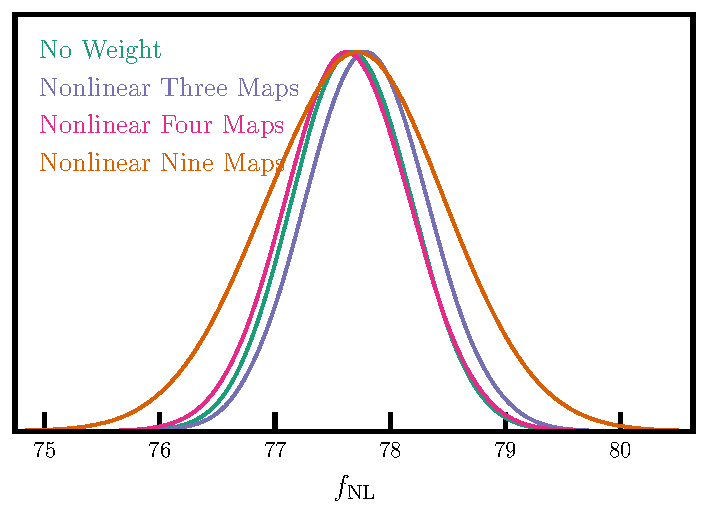
\includegraphics[width=0.45\textwidth]{figures/mcmcp_cont.pdf}
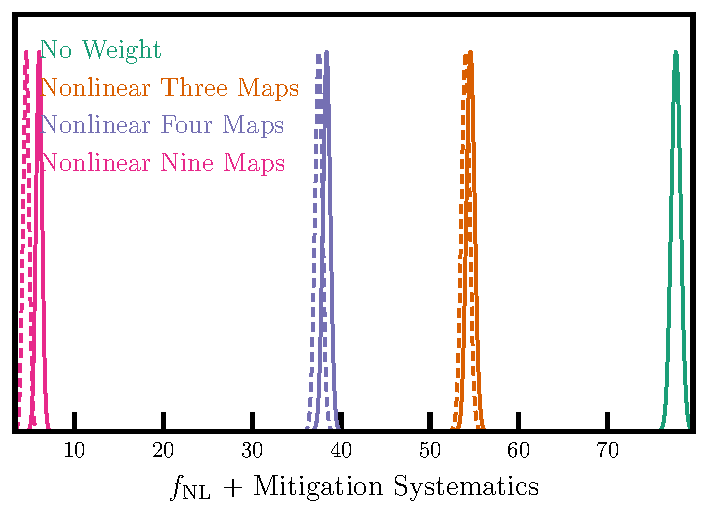
\includegraphics[width=0.45\textwidth]{figures/mcmcp_contnoshift.pdf}
\caption{Probability distributions of $\fnl$ from the mean power spectrum of the $\fnl=0$ (top) and $\fnl=76.9$ (bottom) mocks before and after mitigation with the non-linear methods using three, four, and nine maps. The dashed (solid) curves show the distributions for the contaminated (clean) mocks. Left: The posteriors are adjusted to account for the over-correction effect. Right: The posteriors are subject to the over-correction effect, and thus the scaling of $\fnl$ values is biased due to mitigation.}\label{fig:contmcmc}
\end{figure*}


% \section{Redshift distribution}
% Redshift distribution of LRGs is constructed from the DESI SV data release of Denali with the same selection. The fiducial distribution only covers the redshift range from 0.2 to 1.35. Below we test the impact of LRG dN/dz on the angular power spectrum.


% \begin{figure}
% \centering
% 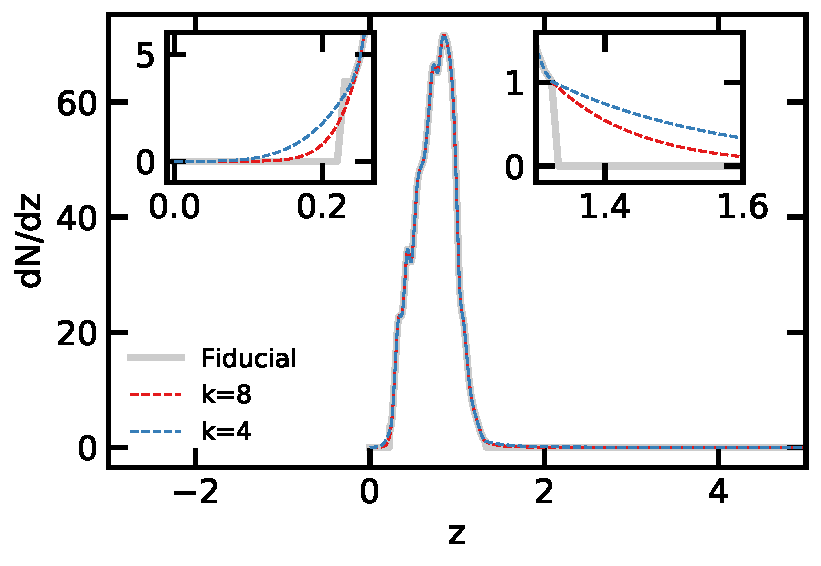
\includegraphics[width=0.45\textwidth]{nztreat.pdf}
% 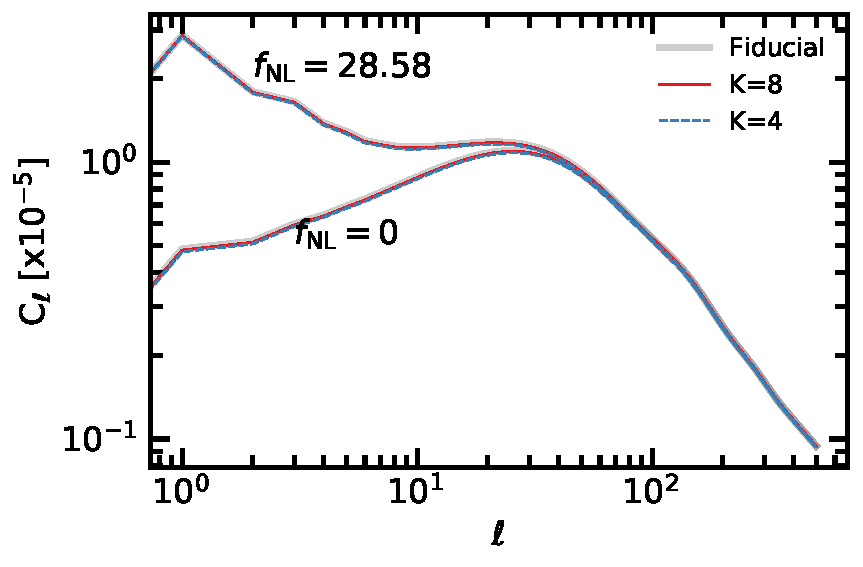
\includegraphics[width=0.45\textwidth]{cell_nz.pdf}
% \caption{Top: Redshift distribution of LRGs. Bottom: Power spectrum given various dN/dz treatments for two arbitrary $\fnl$ values.}
% \end{figure}